% This must be in the first 5 lines to tell arXiv to use pdfLaTeX, which is strongly recommended.
\pdfoutput=1
% In particular, the hyperref package requires pdfLaTeX in order to break URLs across lines.

\documentclass[11pt]{article}

% Remove the "review" option to generate the final version.
\usepackage{acl}
\usepackage{graphicx}
\graphicspath{ {./narrative_eye_tracking_analysis/images/} }
% Standard package includes
\usepackage{times}
\usepackage{latexsym}

% For proper rendering and hyphenation of words containing Latin characters (including in bib files)
\usepackage[T1]{fontenc}
% For Vietnamese characters
% \usepackage[T5]{fontenc}
% See https://www.latex-project.org/help/documentation/encguide.pdf for other character sets

% This assumes your files are encoded as UTF8
\usepackage[utf8]{inputenc}

% This is not strictly necessary, and may be commented out,
% but it will improve the layout of the manuscript,
% and will typically save some space.
\usepackage{microtype}

% If the title and author information does not fit in the area allocated, uncomment the following
%
%\setlength\titlebox{<dim>}
%
% and set <dim> to something 5cm or larger.

\title{Instructions for *ACL Proceedings}

% Author information can be set in various styles:
% For several authors from the same institution:
% \author{Author 1 \and ... \and Author n \\
%         Address line \\ ... \\ Address line}
% if the names do not fit well on one line use
%         Author 1 \\ {\bf Author 2} \\ ... \\ {\bf Author n} \\
% For authors from different institutions:
% \author{Author 1 \\ Address line \\  ... \\ Address line
%         \And  ... \And
%         Author n \\ Address line \\ ... \\ Address line}
% To start a seperate ``row'' of authors use \AND, as in
% \author{Author 1 \\ Address line \\  ... \\ Address line
%         \AND
%         Author 2 \\ Address line \\ ... \\ Address line \And
%         Author 3 \\ Address line \\ ... \\ Address line}

\author{First Author \\
  Affiliation / Address line 1 \\
  Affiliation / Address line 2 \\
  Affiliation / Address line 3 \\
  \texttt{email@domain} \\\And
  Second Author \\
  Affiliation / Address line 1 \\
  Affiliation / Address line 2 \\
  Affiliation / Address line 3 \\
  \texttt{email@domain} \\}

\begin{document}
\maketitle
\begin{abstract}
Capturing readers' engagement in fiction is a challenging but important aspect of narrative understanding. In this study, we collected 23 readers’ reactions to 2 short stories through eye tracking, sentence-level annotations, and an overall engagement scale survey. Our aim is to analyze the significance of various qualities of the text in predicting how engaging a reader is likely to find it. As enjoyment of fiction is highly contextual, we will also investigate individual differences in our data. Furthering our understanding of what captivates readers in fiction will help better inform models used in creative narrative generation and collaborative writing tools.

\end{abstract}

\section{Introduction}

The question of reader engagement in fiction has been studied in the psychology field for decades, with some of the foundational theoretical work from Iser (citation needed) and Gerrig paving the way for more recent theoretical frameworks and experimental setups, which started in the early 2000s with the work by Green (citation) in the field of Media Psychology. In the past ten years, this question has been picked up in more fields, such as cognitive science, psycholinguistics, and computational narrative understanding.

However, as Jacobs emphasized (2018), the samples normally collected are small and not enough to compensate for individual differences in reading patterns due to reader context, among other factors. In order to help close the experimental gap, one contribution of this study is to provide the computational community with a data set of reader reactions to literary short fiction, which Jacobs refers to as "hot" experimental research. This is opposed to setups in which the stories are contrived for the purpose of the study.

Green's 2006 study narrowed down the salient aspects of reader engagement to create narrative engagement scale, which we have modified slightly to gage overall interest in the story. In addition, in order to obtain more granular information, we used these aspects to design an annotation task that would provide sentence-level feedback.

\section{Related Research}

[See Table 1 for comparison matrix. Brief description of other experimental setups and conclusions]

\begin{table*}[t]
\centering
\begin{tabular}{|c|c|c|c|c|c|c|}
\hline
& \textbf{Ours} & \textbf{Kunz et al.} & \textbf{Mangen et al.} & \textbf{Hsu et al.} & \textbf{Mak et al.} & \textbf{Maslej et al.} \\
\hline
\multicolumn{7}{|l|}{\textbf{Data gathered}}\\\hline
Eye tracking & x & x & x &  & x &  \\\hline
Saccade angle &  & x & x &  &  & \\\hline
fMRI &  &  &  & x &  & \\\hline
Engagement survey & x & x & x &  & x & x\\\hline
Engagement annotation & x &  &  & x &  & \\\hline
\multicolumn{7}{|l|}{\textbf{Textual features extracted}}\\\hline
Emotional arc & x &  &  &  &  & \\\hline
Lexical categories & x &  &  & x &  & x\\\hline
Description category &  &  & x &  &  & \\\hline

\end{tabular}
\caption{Comparison between our study and other similar experiments.}
\label{tab:accents}
\end{table*}

\section{Research questions}

\subsection{RQ1: Does absorption in a story lead to longer gaze durations?}

Subquestion: do “Present” highlights (i.e. transported) correlate with faster reading and “Connected” and “Curious” highlights with slower reading as the Jacobs model hypothesized?

\subsection{RQ2: (move to future work) Does gaze duration increase in foregrounding passages and decrease in backgrounding passages?}

Subquestion: is absorption greater in foregrounding passages?

\subsection{RQ3: How much is engagement dependent on reader context vs. linguistic (discourse) features?}

What are the overlapping cases (sentences) when those two sets of features agree? What are the diverging cases? Can discourse features be used as a proxy for predicting eye-tracking features?

\subsection{RQ4: Are eye-tracking patterns consistent across users?}

If they are consistent, can we build a model using all of the users’ data to predict the engagement label or their future time-series data? If not, can we build separate models for each user? Analyses on diverging cases between the users: why are they diverging? Perhaps based on background, personal experience, interests, etc.

\subsection{RQ5: Is there a correlation between a sentence having low average word valence and reader’s absorption?}

\subsection{RQ6: Can we predict whether a reader enjoyed the story overall based on eye-tracking data alone?}

\section{Methods}

\subsection{Participant study}

[Description of the eye tracking setup, number of participants - with the breakdown of age and gender, survey, and description of highlighting exercise]

The study asked 31 English speakers (17 female, 11 male, 3 other, 23 native English speakers, average age: 26) were asked to read two short stories by Anton Chekhov while their eyes were tracked, and then answer an engagement scale survey. (Include eye tracker details here from consent form). After reading through both stories, they completed a highlighting exercise where they highlighted areas according to the following categories:

\begin{itemize}
  \item Present: Able to vividly picture the scene in the story
  \item Confused
  \item Curious: Curious about what will happen next
  \item Connected: Connected to the character; able to identify with them or feel their emotions
  \item Other: Enjoyed it for a different reason
\end{itemize}

Due to poor calibration, 8 samples were discarded, leaving 23 (13 female, 8 male, 2 other, 17 native English speakers, average age: 28).
\begin{figure*}
  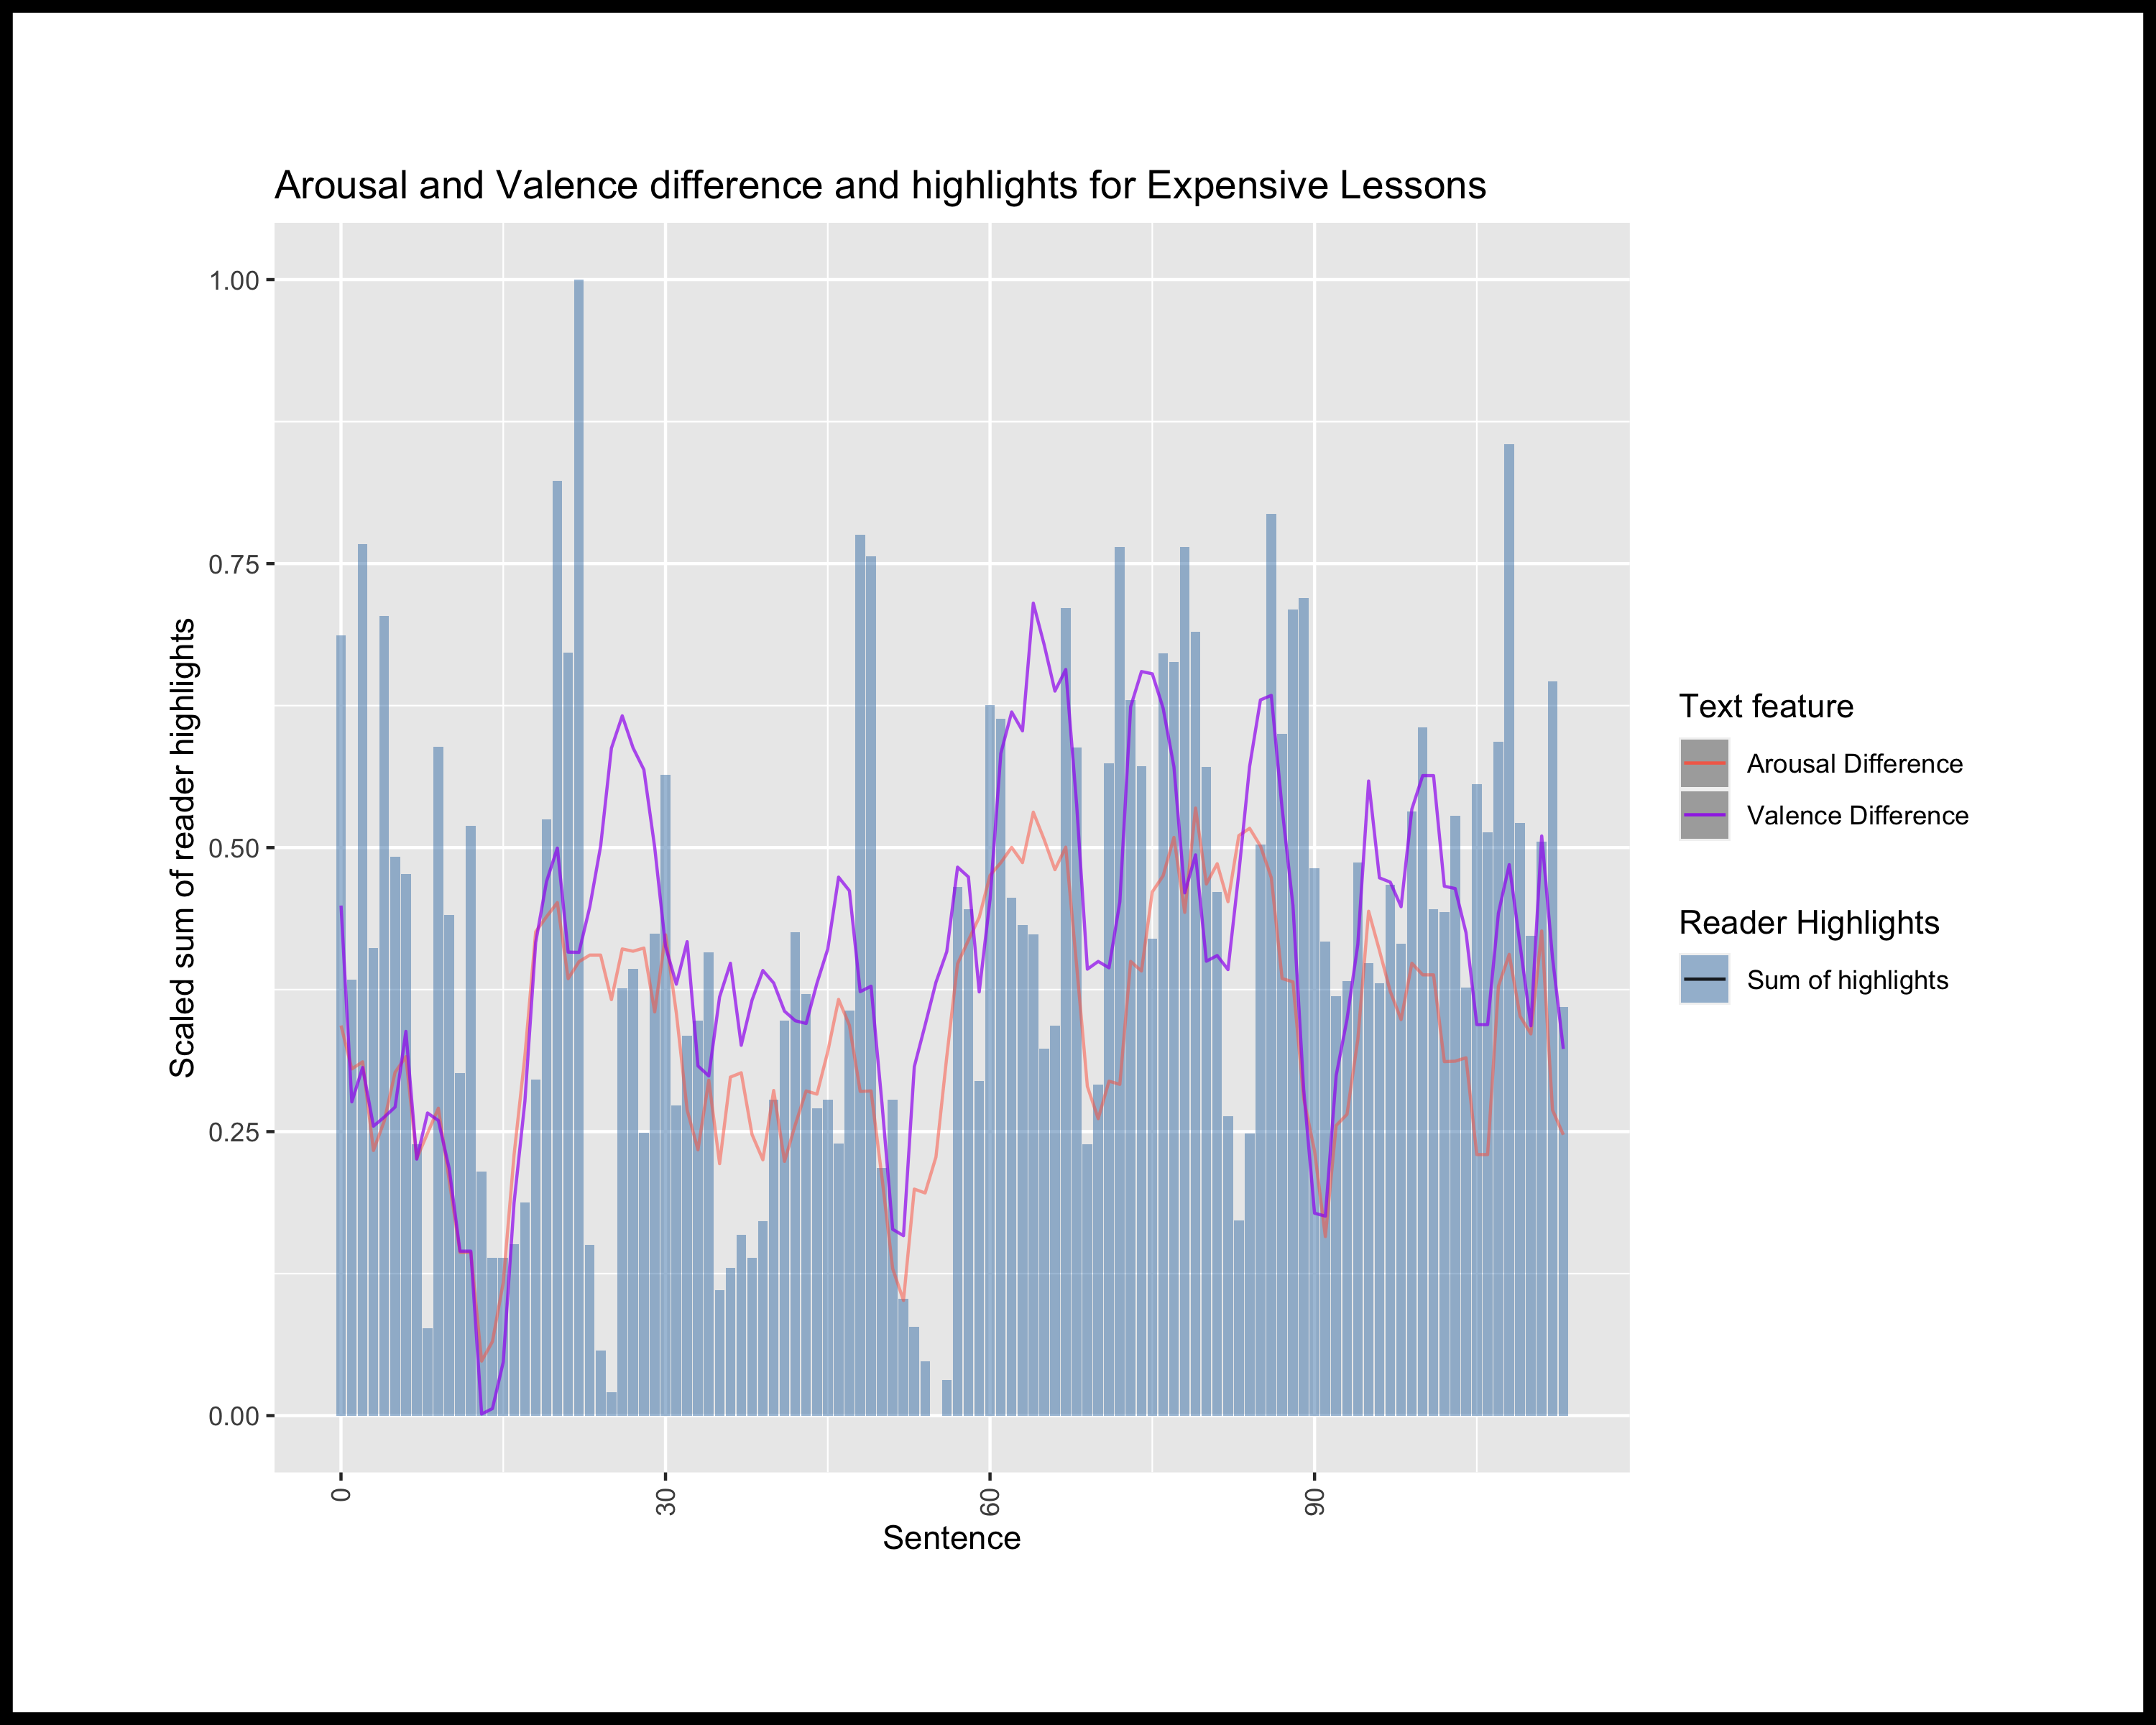
\includegraphics[width=\textwidth,height=10cm]{el_highlights_val_arousal}
  \caption{Plot of valence and arousal of the highlighted sentences.}
\end{figure*}

\subsection{Linguistic and discourse features}

We extracted the following features from the stories to create sentence-level predictors: sentiment scores using the RoBERTa sentiment base model (footnote with link to huggingface), emotion categories using the DistilRoBERTa emotion base model, concreteness from the Brysbaert (brysbaert2014) corpus, valence and arousal from the NRC-VAD corpus, word frequency from the subtlex corpus, and average word length.

\section{Limitations}

[caveat about quality of data and extent of manual drift corrections needed, number of participants, experiment setup getting in the way of genuine absorption, how we filled null values and proportion of sentences with missing data, how many trials were thrown out (6) ..]

\section{Results}

[description of mixed model setup with some results]
"valence (the pleasantness of a stimulus), arousal (the intensity of emotion provoked by a stimulus)" (from norms of valence, arousal, dominance paper)

Other studies have shown that valence and arousal play an important role in predicting interest in a story (Maslej, Jacobs 2015, HSU201596) and Jacobs emphasized the importance of affective and emotional processes. We used linear mixed models to fit predictions of the proportion of the sentence highlighted and gaze duration, with random effects of participant (n=23) and story(n=2). For predicting the proportion of a sentence highlighted, a proxy signifying a higher level of engagement, our results support a slight significance of valence mean (p=0.007), similar to Hsu.

Unlike in other studies, we found that arousal mean had no significance (p=0.598).  However, like Hsu, there was a higher significance for valence-span (p=0.00003) - the difference between valence max and valence min and arousal-span (p=0.00029) - the difference between arousal max and arousal min. This suggests that the reader was more engaged in sentences with a higher range of valence and arousal. This model explains 22.9\% of the variance in the proportion of a sentence highlighted with random effects and 3.7\% without.

In predicting gaze duration, valence mean had a slight significance (p=0.0181) and arousal mean had none (p=0.365) and valence-span (p=0.0336) had a slight significance while arousal-span was found to be significant, but with a negative slope (p=0.00047). These findings do not support Jacobs's proposed framework, which states that passages that engage our emotions would likely result in slower reading. However, we found a positive relationship with negative sentiment (p=0.0048), which may partially support his proposal that the affective mode of reading is more readily triggered by negative emotion. Length of the sentence (p=0.000012) and word frequency (p=0.000048) were the most significant predictors of dwell time. 
\section{Conclusion}


\subsection{References}

\nocite{Green2004,liwc_22,kuzmicova2014,brysbaert2014,chung-fat-yim_cilento_piotrowska_mar_2019,Maslej2019TheTF,boyd_blackburn_pennebaker_2020,green_brock_kaufman_2006,kasunic_kaufman_2018,Consoli2018,busselle2009,jacobs2018,jacobs2017,stockwell2002cognitive,HSU201596,willems_2015,mak2019,kunze2015,ferreira-goncalo-oliveira-2018-seeking,rashkin-etal-2016-connotation,aryani2013,delatorre2019,andrade2020,indico2015}

\bibliographystyle{acl_natbib}
\bibliography{anthology,custom}


\section*{Acknowledgements}

[Text Group for initial feedback on experiment setup, Blue Lantern Writing Group for additional feedback]

\appendix

\section{Example Appendix}
\label{sec:appendix}

[more details on experiment: exact questions asked and instructions? some considerations for future eye tracking studies, such as use mount and make sure text is more spaced out]

\end{document}